\documentclass[12pt,a4paper]{article}
\usepackage[left=20mm,top=20mm,total={170mm,257mm}]{geometry}

%  - documentation minted -
% https://tools.ietf.org/doc/texlive-doc/latex/minted/minted.pdf
% - documentation tcolorbox -
% https://ctan.math.washington.edu/tex-archive/macros/latex/contrib/tcolorbox/tcolorbox.pdf
% - documentation tabular -
% https://mirror.truenetwork.ru/CTAN/macros/latex/contrib/tabularray/tabularray.pdf
% - documentation pgfplots -
% http://www.bakoma-tex.com/doc/latex/pgfplots/pgfplots.pdf

\usepackage{styles/preamble}
\usepackage{minted}                 % Для вставок с кодом
\usemintedstyle{vs}                                     % Стиль кода пакета minted
\usepackage{amsmath}
\usepackage{mathtools}              % Для математических формул
\usepackage{setspace}               % Для междустрочного интервала


\usepackage[dvipsnames]{xcolor}
\setmainfont[Scale=1.0]{Noto Sans}  % Connect font

\definecolor{background-gray}{gray}{1}
\definecolor{mintedbackground}{rgb}{0.98,0.98,0.98}     % Color minted background

\usepackage{pgfplots}
\pgfplotsset{compat=1.17}                                           % Версия pgfplots
\newcommand{\romannumeralcaps}[1]{\MakeUppercase{\romannumeral #1}} % Римские цифры

\usepackage{multicol}           % Мультиколонки
\usepackage{hyperref}           % Для работы с ссылками

% Property for C++ code
\newmintedfile[cppcode]{cpp}{
    bgcolor=background-gray,    % Background
    fontfamily=tt,              % Font
    linenos=true,               % Numbering
    numberblanklines=true,      %
    numbersep=3pt,              % Separator number
    gobble=0,                   % Сожрать первые символы каждой строки
    frame=leftline,             % Left line
    framerule=0.2pt,            % Ширина линии
    framesep=10pt,              % Отступ от разделителя
    funcnamehighlighting=true,  %
    tabsize=4,                  % Количество пробелов табуляции
    mathescape=true,            % Включение математических формул
    showspaces=false,           % Показывать пробелы
    showtabs=false,             % Показывать табуляции
    baselinestretch=1,          % Расстояние между строчками
    breaklines                  % Перенос строк
}

\usepackage[most]{tcolorbox}    % для управления цветом
\newtcolorbox{myquote}{
    colback=background-gray,
    coltext=black,
    grow to right by=-1mm,
    grow to left by=-1mm,
    boxrule=-1mm,
    boxsep=0pt
} % настройки области с изменённым фоном

\usepackage{tabularray}

% =================================================
% НАЧАЛО ДОКУМЕНТА
% =================================================

\begin{document}
\import{titlepage/}{title}

\section{Условие задачи}                % Условие задачи
\subsection*{Формулировка задачи}       % Формулировка задачи

МКЭ для двумерной краевой задачи для эллиптического уравнения в декартовой системе
координат. Базисные функции линейные на треугольниках. Краевые условия всех типов.
Коэффициент диффузии $\lambda$ разложить по линейным базисным функциям. Матрицу СЛАУ
генерировать в разреженном строчном формате. Для решения СЛАУ использовать метод
сопряженных градиентов (МСГ) или локально-оптимальную схему (ЛОС) с неполной
факторизацией.

\subsection*{Постановка задачи}

Эллиптическая краевая задача для функции \textit{u}
определяется дифференциальным уравнением:

\[ -div( \lambda \ grad u) + \gamma u = f \]

\noindent заданным в некоторой области $\Omega$ с границей
$S=S_1 \cup S_2 \cup S_3$ и краевыми условиями:

\[ u \vert_{S_1} = u_g \]
\[ \lambda \frac{\partial u}{\partial n} \bigg\vert_{S_2} = \theta \]
\[ \lambda \frac{\partial u}{\partial n} \bigg\vert_{S_3}
    + \beta(u \vert_{S_3} - u_{\beta}) = 0 \]

\noindent В декартовой системе координат {x,y} это
уравнение может быть записано в виде

\[ -\frac{\partial}{\partial x}
    \left( \lambda \frac{\partial u}{\partial x} \right)
    -\frac{\partial}{\partial y}
    \left( \lambda \frac{\partial u}{\partial y} \right)
    + \gamma u = f \]

\noindent Исходное уравнение можно переписать
в виде: $Lu = f$, где $Lu = -div( \lambda grad u) + \gamma u$.

\noindent Тогда чтобы решить исзодную задачу
следует левую и праую части уравнения домножить
на функцию $v$ из пространства пробных функций
и проинтегрировать по $\Omega$. Фактически это
соответсвует скалярному умножению $Lu$ и $f$
на $v$ в пространтсве $L_2(\Omega)$:

\[ (Lu, v) = (f, v) \]
\[ (Lu - f, v) = 0 \]

\noindent Это уравнение Галеркина в слабой форме. \\
В пространстве $L_2(\Omega)$ скалярное произведение
вычисляется по формуле:

\[ (u, v) = \int \limits_{\Omega} uv d\Omega \]

\noindent Перепишем уравнение Галеркина в явном виде:

\[
    -\int \limits_{\Omega} div(\lambda \ grad u) v \ d\Omega
    +\int \limits_{\Omega} \gamma u v \ d\Omega
    -\int \limits_{\Omega} fv \ d\Omega
    = 0
\]

\noindent Воспользуемся формулой Грина:

\[
    \int \limits_{\Omega} (\lambda \ grad u \ grad v) \ d\Omega
    = -\int \limits_{\Omega} div (\lambda \ grad u) v \ d\Omega
    + \int \limits_S \lambda \frac{\partial u}{\partial n} v \ dS
\]

\noindent Сделав соответствующую подстановку,
получим уравнение вида:

\[
    \int \limits_{\Omega} (\lambda \ grad u \ grad v) d\Omega
    - \int \limits_S \lambda \frac{\partial u}{\partial n} v dS
    + \int \limits_{\Omega} \gamma u v \ d\Omega
    \int \limits_{\Omega} f v \ d\Omega
    = 0
\]

\noindent Учитывая краевые условия  $S=S_1 \cup S_2 \cup S_3$, получим:

\[
    \int \limits_{\Omega} (\lambda \ grad u \ grad v) d\Omega
    - \int \limits_{S_1} \lambda \frac{\partial u}{\partial n} v dS
    - \int \limits_{S_2} \theta v dS
    - \int \limits_{S_3} \beta(u \vert_{\beta} - u) v dS
    + \int \limits_{\Omega} \gamma u v \ d\Omega
    - \int \limits_{\Omega} f v \ d\Omega
    = 0
\]

\noindent Так как $v \vert_{S_1} = 0$, то
\[
    \int \limits_{S_1} \lambda \frac{\partial u}{\partial n} v \ dS = 0
\]
\noindent Уравнение примет вид:

\[
    \int \limits_{\Omega} (\lambda grad u \text{ } grad v) d\Omega
    + \int \limits_{S_3} \beta u v dS
    + \int \limits_{\Omega} \gamma u v d\Omega
    =
    \int \limits_{S_2} \theta v dS
    + \int \limits_{S_3} \beta u \vert_{\beta} v dS
    + \int \limits_{\Omega} f v d\Omega
    = 0
\]

\noindent Будем искать решение в виде:

\[
    u = \sum \limits_{i=1}^n q_i \psi_i
\]

\noindent где $\psi_i$ - базисные функции. Функция $v$ может
быть представлена в таком же виде. Подставив, получим СЛАУ
для компонент $q_i$:

\begin{eqnarray*}
    \sum \limits_{i=1}^n q_i \left(
        \int \limits_{\Omega} (\lambda \ grad \psi_i \ grad \psi_j) d\Omega
        + \int \limits_{S_3} \beta \psi_i \psi_j \ dS
        + \int \limits_{\Omega} \gamma \psi_i \psi_j \ d\Omega
    \right)
    = \\
    =
    \int \limits_{S_2} \theta \psi_j \ dS
    + \int \limits_{S_3} \beta u_{\beta} \psi_j \ dS
    + \int \limits_{\Omega} f \psi_j \ d\Omega
\end{eqnarray*}


\begin{spacing}{1.25}
    \noindent Поскольку исходная задача рассматривается в
    декартовой системе координат, то
    $grad u = \left( \frac{\partial u}{\partial x}, \frac{\partial u}{\partial y} \right)$
    и, соответсвенно:
    $
    grad u \text{ } grad v =
    \frac{\partial u}{\partial x}
    \frac{\partial u}{\partial x}
    +
    \frac{\partial u}{\partial y}
    \frac{\partial u}{\partial y}
    $.
    Отсюда получаем уравнение в виде:
\end{spacing}


\begin{eqnarray*}
    \sum \limits_{j=1}^n q_j \int \limits_{\Omega}
    \lambda \left(
        \frac{\partial \psi_j}{\partial x} \frac{\partial \psi_i}{\partial x}
        +
        \frac{\partial \psi_j}{\partial y} \frac{\partial \psi_i}{\partial y}
    \right)
    dxdy
    +
    \sum \limits_{j=1}^n q_j \int \limits_{\Omega}
    \gamma \psi_j \psi_i \ dxdy
    +
    \sum \limits_{j=1}^n q_j \int \limits_{\Omega}
    \beta \psi_j \psi_i \ dxdy
    = \\
    =
    \int \limits_{\Omega} f \psi_i \ dxdy
    +
    \int \limits_{S_2} \theta \psi_i \ dxdy
    +
    \int \limits_{S_3} \beta u_{\beta} \psi_i \ dxdy
\end{eqnarray*}


\subsection*{Конечноэлементная дискретизация}

Так как для решения задачи используются линейные базисные
функции, то на каждом конечном элементе $\Omega_k$ -
треугольнике эти функции будут совпадать с функциями
$L_1(x,y), L_2(x,y), L_3(x,y)$, такими, что $L_1(x,y)$
равна единице в вершине $(x_1,y_1)$ и нулю во всех остальных
вершинах, $L_2(x,y)$ равна единице в вершине $(x_2,y_2)$
и нулю во всех остальных вершинах, $L_3(x,y)$ равна единице
в вершине $(x_3,y_3)$ и нулю во всех остальных вершинах.
Любая линейная на $\Omega_k$ функция представима в виде
линейной комбинации этих базисных линейных функций,
коэффициентами будут значения функции в каждой из вершин
треугольника $\Omega_k$. Таким образом, на каждом конечном
элементе нам понадобятся три узла – вершины треугольника.

\[ \psi_1 = L_1(x,y) \]
\[ \psi_2 = L_2(x,y) \]
\[ \psi_3 = L_3(x,y) \]

\noindent Учитывая построение \textit{L-функций},
получаем следующие соотношения:

\begin{equation*}
    \begin{cases}
        L_1 + L_2 + L_3 = 1          \\
        L_1x_1 + L_2x_2 + L_3x_3 = x \\
        L_1y_1 + L_2y_2 + L_3y_3 = y
    \end{cases}
\end{equation*}

\noindent Т.e. имеем систему:
\renewcommand{\arraystretch}{1.25}
\begin{equation*}
    \begin{pmatrix}
        1   & 1   & 1   \\
        x_1 & x_2 & x_3 \\
        y_1 & y_2 & y_3
    \end{pmatrix}
    \cdot
    \begin{pmatrix}
        L_1 \\
        L_2 \\
        L_3
    \end{pmatrix}
    =
    \begin{pmatrix}
        1 \\
        x \\
        y
    \end{pmatrix}
\end{equation*}
\renewcommand{\arraystretch}{1.0}

\noindent Отсюда находим коэффициенты
линейных функций $L_1(x,y), L_2(x,y), L_3(x,y)$
\[ L_i = a_0^i + a_1^ix + a_2^iy, i = \overline{1,3} \]

\renewcommand{\arraystretch}{1.25}
\begin{equation*}
    \begin{pmatrix}
        \alpha_0^1 & \alpha_1^1 & \alpha_2^1 \\
        \alpha_0^2 & \alpha_1^2 & \alpha_2^2 \\
        \alpha_0^3 & \alpha_1^3 & \alpha_2^3
    \end{pmatrix}
    =
    D^{-1}
    =
    {\begin{pmatrix}
        1   & 1   & 1   \\
        x_1 & x_2 & x_3 \\
        y_1 & y_2 & y_3
    \end{pmatrix}}^{-1}
\end{equation*}
\renewcommand{\arraystretch}{1.0}

\renewcommand{\arraystretch}{1.25}
\begin{equation*}
    D^{-1} = \frac{1}{\vert det D \vert}
    \begin{pmatrix}
        x_2y_3-x_3y_2 & y_2-y_3 & x_3-x_2 \\
        x_3y_1-x_1y_3 & y_3-y_1 & x_1-x_3 \\
        x_1y_2-x_2y_1 & y_1-y_2 & x_2-x_1
    \end{pmatrix}
\end{equation*}
\renewcommand{\arraystretch}{1.0}

\subsection*{Переход к локальным матрицам}

Чтобы получить выражения для локальных
матриц жёсткости G и массы M каждого
конечного элемента $\Omega_K$, перейдём
к решению локальной задачи на каждом
конечном элементе. Полученное уравнение
для области $\Omega$ представим в виде
суммы интегралов по областям $\Omega_k$
без учёта краевых условий. Тогда на
каждом конечном элементе будем решать
локальную задачу построения матриц
жёсткости, массы и вектора правой части.

$$
\int \limits_{\Omega_k} \lambda
\left(
    \frac{\partial \psi_j}{\partial x}
    \frac{\partial \psi_i}{\partial x}
    +
    \frac{\partial \psi_j}{\partial y}
    \frac{\partial \psi_i}{\partial y}
\right) dxdy
+
\int \limits_{\Omega_k} \gamma \psi_j \psi_i dsdy
=
\int \limits_{\Omega_k} f \psi_i dxdy
$$

\noindent Локальная матрица будет представлять
собой сумму матриц жёсткости и массы и будет
иметь размерность $3 \times 3$ (по числу
узлов на конечном элементе)

\subsection*{Построение матрицы массы}

\begin{eqnarray*}
M_{ij} =
    \int \limits_{\Omega_m} \gamma Y_iY_j d\Omega_m =
    \Big \vert \gamma = Y_1\gamma_1
                      + Y_2\gamma_2
                      + Y_3\gamma_3
    \Big \vert
    =
    \int \limits_{\Omega_m}
        \left(
            Y_1\gamma_1
          + Y_2\gamma_2
          + Y_3\gamma_3
        \right) Y_i Y_j d \Omega_m = \\ =
    \gamma_1 \int \limits_{\Omega_m} Y_1 Y_i Y_j d \Omega_m +
    \gamma_2 \int \limits_{\Omega_m} Y_2 Y_i Y_j d \Omega_m +
    \gamma_3 \int \limits_{\Omega_m} Y_3 Y_i Y_j d \Omega_m = \\ =
    \gamma_1 \int \limits_{\Omega_m} L_1 L_i L_j d \Omega_m +
    \gamma_2 \int \limits_{\Omega_m} L_2 L_i L_j d \Omega_m +
    \gamma_3 \int \limits_{\Omega_m} L_3 L_i L_j d \Omega_m
\end{eqnarray*}

\subsection*{Построение матрицы жёсткости}

Рассмотрим первый член в выражении для k-го конечного
эдемента:

$$
\int \limits_{\Omega_k} \lambda
    \left(
        \frac{\partial \psi_j}{\partial x}
        \frac{\partial \psi_i}{\partial x}
        +
        \frac{\partial \psi_j}{\partial y}
        \frac{\partial \psi_i}{\partial y}
        dxdy
    \right)
$$

$$
B_{i,j}=(\alpha_1^i \alpha_1^j + \alpha_2^i \alpha_2^j)
    \frac{\big \vert det D \big \vert}{2}
    \hspace{15pt} i,j=\overline{0,2}
$$

\subsection*{Построение вектора правой части}

Рассмотрим правую часть выражения для k-го конечного элемента:

$$
\int \limits_{\Omega_k} f \psi_i dxdy
$$

\noindent представим $f$ в виде $f_1 L_1 + f_2 L_2 + f_3 L_3$, где
$f_i$ - значения в вершинах треугольника. Получим:

$$
\int \limits_{\Omega_k} f_q L_q L_i dxdy =
    f_q \int \limits_{\Omega_k} L_q L_i d \Omega_k
$$

\noindent Таким образом:
$$
G_i = \sum \limits_{q=1}^{3}
    f_q \int \limits_{\Omega_k} L_q L_i d\Omega_k
    \hspace{15pt} i=\overline{0,2}
$$

\subsection*{Сборка глобальной матрицы и глобального вектора}

При формировании глобальной матрицы из локальных,
полученных суммированием соответствующих матриц
массы и жесткости, учитываем соответствие локальной
и глобальной нумераций каждого конечного элемента.
Глобальная нумерация каждого конечного элемента
однозначно определяет позиции вклада его локальной м
атрицы в глобальную. Поэтому, зная глобальные
номера соответствующих узлов конечного элемента,
определяем и то, какие элементы глобальной матрицы
изменятся при учете текущего конечного элемента.
Аналогичным образом определяется вклад локального
вектора правой части в глобальный. При учете
текущего локального вектора изменятся те элементы
глобального вектора правой части, номера которых
совпадают с глобальными номерами узлов, присутствующих
в этом конечном элементе.

\subsection*{Учёт первых краевых условий}

Для учета первых краевых условий, в глобальной матрице
и глобальном векторе находим соответствующую глобальному
номеру краевого узла строку и зануляем всё кроме
диагонального элемента, которому присваиваем 1, а вместо
элемента с таким номером в векторе правой части - значение
краевого условия, заданное в исходной задаче.


\subsection*{Учёт вторых и трeтьих краевых условий}

Рассмотрим краевые условия второго и третьего рода:
$$
    \lambda \frac{\partial u}{\partial n}
    \bigg\vert_{S_2} = \theta
$$

$$
    \lambda \frac{\partial u}{\partial n}
    \bigg\vert_{S_3} +
    \beta(u \vert_{S_3} - u_{\beta}) = 0
$$

\noindent Отсюда получаем, что для учёта краевых условий
необходимо вычислить интегралы:

$$
    \int \limits_{S_2} \theta \psi_j dxdy,          \hspace{25pt}
    \int \limits_{S_3} \beta u_{\beta} \psi_j dxdy, \hspace{25pt}
    \int \limits_{S_3} \beta \psi_i \psi_j dxdy
$$

\noindent Краевые условия второго и третьего рода задаются
на рёбрах, т.е. определяются двумя узлами, лежащими на
ребру. Будем считать, что параметр $\beta$ на $S_3$
постоянен, тогда параметр $г_{\beta}$ будем
раскладывать по двум базисным функциям,
определённым на этом ребре:
$$ u_{\beta} = u_{\beta 1} \phi_1 + u_{\beta 2} \phi_2 $$


\noindent где $\phi_i, \hspace{5pt} i=\overline{0,1}$
- локально занумерованные линейные базисные функции,
которые имеют также свои глобальные номера во всей
расчетной области, а $u_{\beta i}$ - значение функции
$u_{\beta}$ в узлах ребра. \\

\noindent Аналогично поступаем и при учете вторых
краевых условий, раскладывая по базису ребра функцию
$\theta = \theta_0 \phi_0 + theta_1 \phi_1$.

\noindent Тогда приведенные выше интегралы примут вид:

$$ I_1 = \int \limits_{S_2} (\theta_0 \phi_0 + \theta_1 \phi_1) \phi_i dxdy $$
$$ I_2 = \beta \int \limits_{S_3} (u_{\beta 1} \phi_0 + u_{\beta 2} \phi_1) \phi_i dxdy $$
$$ I_3 = \beta \int \limits_{S_3} \phi_i \phi_j dxdy $$

\noindent Фактически, решая задачу учета краевых условий второго
и третьего рода, мы переходим к решению одномерной
задачи на ребре для того, чтобы занести соответствующие
результаты в глобальную матрицу и вектор. \\

\noindent Базисными функциями ребра являются две
ненулевые на данном ребре базисные функции из
$\phi_i, \hspace{5pt} i=\overline{0,1}$
конечного элемента. \\

\noindent Для учёта вклада вторых и третьих краевых условий
рассчитываются 2 матрицы $2 \times 2$. \\

\noindent Игтегралы $I_1, I_2, I_3$ будем вычислять по формуле:
$$
    \int \limits_Г (L_i)^{v_i} (L_j)^{v_j} dS =
    \frac{v_i ! v_j !}{(v_i + v_j + 1)!} mes \varGamma,
    \hspace{5pt} i \neq j
$$

\noindent где $mes \varGamma$ длина ребра. При этом независимо
от того, что на каждом из ребер присутствуют свои функции,
интегралы, посчитанные по приведенным выше формулам,
будут равны.

\renewcommand{\arraystretch}{1.25}
\begin{equation*}
    I_1 =
    \begin{pmatrix}
        \int \limits_{S_2} L_1L_1dxdy & \int \limits_{S_2} L_1L_2dxdy \\
        \int \limits_{S_2} L_2L_1dxdy & \int \limits_{S_2} L_2L_2dxdy
    \end{pmatrix}
    \begin{pmatrix}
        \theta_1 \\
        \theta_2
    \end{pmatrix}
    = \frac{1}{6} mes S_2
    \begin{pmatrix}
        2 & 1 \\
        1 & 2
    \end{pmatrix}
    \begin{pmatrix}
        \theta_1 \\
        \theta_2
    \end{pmatrix}
\end{equation*}
\renewcommand{\arraystretch}{1.0}

\noindent Этот вектор поправок в правую
часть позволяет учесть не только вторые
краевые условия, но и часть
$\beta u_{\beta}$ из третьих.
Осталось рассмотреть матрицу
поправок в левую часть:
$$
I_3 = \beta \int \limits_{S_3}
\phi_i \phi_j dxdy
$$

\noindent Очевидно, что получится та же
матрица, только не умноженная на вектор
констант.

$$
I_3 = \frac{1}{6} mes S_3
\begin{pmatrix}
    2 & 1 \\
    1 & 2
\end{pmatrix}
$$

\noindent Добавляя эту матрицу в левую часть,
на места соответствующие номерам узлов,
получаем учет третьих краевых условий.


\newpage
\section{Текст программы}

Весь проект:
\href{https://github.com/ISTECTION/FEM}{https://github.com/ISTECTION/FEM}

\begin{myquote}
    \begin{center}
        \textbf{main.cpp}
    \end{center}
\end{myquote}
\cppcode{source/main.cpp}

\begin{myquote}
    \begin{center}
        \textbf{Union.hpp}
    \end{center}
\end{myquote}
\cppcode{source/Union.hpp}

\begin{myquote}
    \begin{center}
        \textbf{FEM.hpp}
    \end{center}
\end{myquote}
\cppcode{source/FEM.hpp}

\begin{myquote}
    \begin{center}
        \textbf{Data.hpp}
    \end{center}
\end{myquote}
\cppcode{source/Data.hpp}

\begin{myquote}
    \begin{center}
        \textbf{LOS.hpp}
    \end{center}
\end{myquote}
\cppcode{source/LOS.hpp}

\begin{myquote}
    \begin{center}
        \textbf{LOS\_Function.hpp}
    \end{center}
\end{myquote}
\cppcode{source/LOS_Function.hpp}

\begin{myquote}
    \begin{center}
        \textbf{lightweight.hpp}
    \end{center}
\end{myquote}
\cppcode{source/lightweight.hpp}

\begin{myquote}
    \begin{center}
        \textbf{overload.hpp}
    \end{center}
\end{myquote}
\cppcode{source/overload.hpp}

% Тестирование
\section{Тестирование}

\subsection*{Тест №1}

\setlength{\columnsep}{-4.5cm}
\begin{multicols}{2}

    \setlength{\leftskip}{2.5cm}
    \noindent   \vspace{5mm} \\
    $u(x,y)=1$  \vspace{2mm} \\
    $f(x,y)=0$  \vspace{2mm} \\
    $\lambda=1$ \vspace{2mm} \\
    $\gamma=0$  \vspace{2mm} \\
    $\beta=0$   \vspace{2mm} \\

    \columnbreak
    \setlength{\leftskip}{2.25cm}
    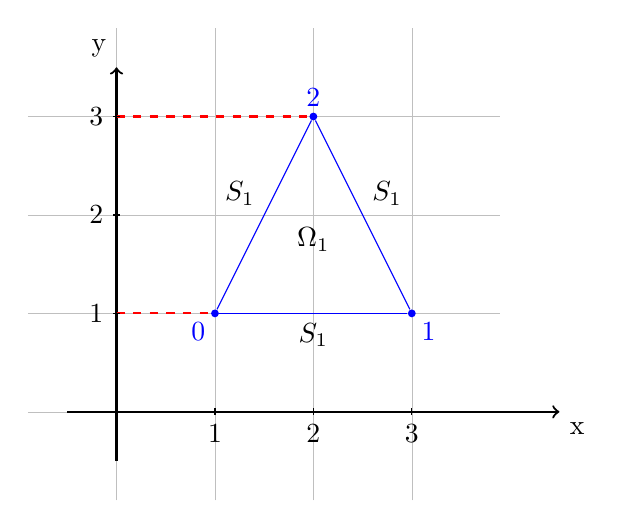
\begin{tikzpicture}[scale=1.25]
        \draw[step=1cm,lightgray,very thin] (-0.9,-0.9) grid (3.9,3.9);     % Сетка

        \draw[thick,->] (-0.5,0) -- (4.5,0) node[anchor=north west] {x};    % Ось X
        \draw[thick,->] (0,-0.5) -- (0,3.5) node[anchor=south east] {y};    % Ось Y

        % Красные пунктирные линии
        \draw[thick, dashed, red] (0,3) -- (2,3);
        \draw[thick, dashed, red] (0,1) -- (1,1);

        % Узлы
        \node[fill=blue, circle, inner sep=1pt, minimum size=1pt] (A) at (1,1){};
        \node[fill=blue, circle, inner sep=1pt, minimum size=1pt] (B) at (3,1){};
        \node[fill=blue, circle, inner sep=1pt, minimum size=1pt] (C) at (2,3){};

        % Подписи узлов
        \node[below left]  at (1,1){\color{blue}$0$};
        \node[below right] at (3,1){\color{blue}$1$};
        \node[above]       at (2,3){\color{blue}$2$};

        % Линии с подписями
        \draw[blue] (A) -- (B) node [midway, below, black] {$S_1$};
        \draw[blue] (B) -- (C) node [midway, above right, black] {$S_1$};
        \draw[blue] (C) -- (A) node [midway, above left, black] {$S_1$};

        % Области
        \node at (2,1.75) {$\Omega_1$};

        % Координаты осей
        \foreach \x in {1,2,3} \draw (\x cm,1pt) -- (\x cm,-1pt) node[anchor=north] {$\x$};
        \foreach \y in {1,2,3} \draw (1pt,\y cm) -- (-1pt,\y cm) node[anchor=east] {$\y$};
    \end{tikzpicture}
\end{multicols}

\setlength{\columnsep}{-2.0cm}
\begin{multicols}{2}
    \setlength{\leftskip}{2.5cm}
    \noindent   \vspace{5mm} \\
    $\romannumeralcaps{1}_0 = 1$

    \columnbreak
    \setlength{\leftskip}{1cm}
    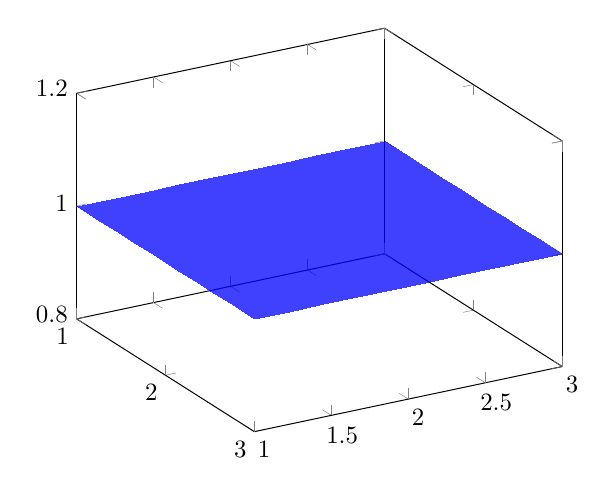
\begin{tikzpicture}[scale=0.9]
        \begin{axis}[view={60}{30}]
            \addplot3[
                surf,
                domain=1:3,
                samples=10,
                fill opacity=0.75,
                shader=interp
            ]
            {1};
        \end{axis}
    \end{tikzpicture}
\end{multicols}

\setlength{\columnsep}{-2.0cm}
\begin{multicols}{2}
    \begin{tblr}{vline{1-5}={0mm,solid},
        row{odd}={bg=azure9},
        row{1}={bg=azure3,fg=white,font=\sffamily}}
        \hline[1.25pt]
        nodes & elems & area & bords     \\
        \hline
        1 1   & 0 1 2 & 0    & 0 0 1 1 0 \\
        3 1   &       &      & 0 1 2 1 0 \\
        2 3   &       &      & 0 2 0 1 0 \\
        \hline[1.25pt]
    \end{tblr}

    \columnbreak
    \setlength{\leftskip}{1cm}
    \begin{tblr}{vline{1-5} = {0mm,solid},
        row{odd}={bg=azure9},
        row{1}={bg=azure3,fg=white,font=\sffamily}}
        \hline[1.25pt]
        $x$ & $x^*$ & $x^*-x$ & $\|x^*-x\|$ \\
        1.000 & 1.000 & 0.00E+00 &          \\
        1.000 & 1.000 & 0.00E+00 & 0.00E+00 \\
        1.000 & 1.000 & 0.00E+00 &          \\
        \hline[1.25pt]
    \end{tblr}
\end{multicols}

\newpage
\subsection*{Тест №2}
\subsubsection*{Количество елементов - 2}

\setlength{\columnsep}{-4.5cm}
\begin{multicols}{2}

    \setlength{\leftskip}{2.5cm}
    \noindent   \vspace{5mm} \\
    $u(x,y)=5x+2y$  \vspace{2mm} \\
    $f(x,y)=10x+4y$ \vspace{2mm} \\
    $\lambda=2$ \vspace{2mm} \\
    $\gamma=2$  \vspace{2mm} \\
    $\beta=5$   \vspace{2mm} \\

    \columnbreak
    \setlength{\leftskip}{2.25cm}
    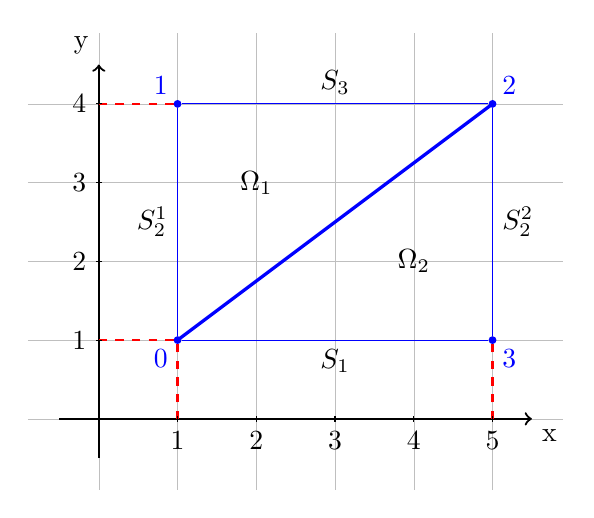
\begin{tikzpicture}[scale=1.0]
        \draw[step=1cm,lightgray,very thin] (-0.9,-0.9) grid (5.9,4.9);

        \draw[thick,->] (-0.5,0) -- (5.5,0) node[anchor=north west] {x};
        \draw[thick,->] (0,-0.5) -- (0,4.5) node[anchor=south east] {y};

        % Красные пунктирные линии
        \draw[thick, dashed, red] (1,0) -- (1,1);
        \draw[thick, dashed, red] (5,0) -- (5,1);
        \draw[thick, dashed, red] (0,1) -- (1,1);
        \draw[thick, dashed, red] (0,4) -- (1,4);

        % Узлы
        \node[fill=blue, circle, inner sep=1pt, minimum size=1pt] (A) at (1,1){};
        \node[fill=blue, circle, inner sep=1pt, minimum size=1pt] (B) at (5,1){};
        \node[fill=blue, circle, inner sep=1pt, minimum size=1pt] (C) at (5,4){};
        \node[fill=blue, circle, inner sep=1pt, minimum size=1pt] (D) at (1,4){};

        % Подписи узлов
        \node[below left]  at (1,1) {\color{blue}$0$};
        \node[above left]  at (1,4) {\color{blue}$1$};
        \node[above right] at (5,4) {\color{blue}$2$};
        \node[below right] at (5,1) {\color{blue}$3$};

        % Линии с подписями
        \draw[blue] (A) -- (B) node [midway, below, black] {$S_1$};
        \draw[blue] (A) -- (D) node [midway, left , black] {$S_2^1$};
        \draw[blue] (B) -- (C) node [midway, right, black] {$S_2^2$};
        \draw[blue] (D) -- (C) node [midway, above, black] {$S_3$};
        \draw[very thick, blue] (1,1) -- (5,4);

        % Области
        \node at (2,3) {$\Omega_1$};
        \node at (4,2) {$\Omega_2$};

        % Координаты осей
        \foreach \x in {1,2,3,4,5} \draw (\x cm,1pt) -- (\x cm,-1pt) node[anchor=north] {$\x$};
        \foreach \y in {1,2,3,4} \draw (1pt,\y cm) -- (-1pt,\y cm) node[anchor=east] {$\y$};
    \end{tikzpicture}
\end{multicols}



\setlength{\columnsep}{-2.0cm}
\begin{multicols}{2}
    \setlength{\leftskip}{2.5cm}
    \noindent   \vspace{5mm} \\
    $\romannumeralcaps{1}_0 = 5x + 2$ \\
    $\romannumeralcaps{2}_0 = -10$    \\
    $\romannumeralcaps{2}_1 = 10$     \\
    $\romannumeralcaps{3}_0 = 5x + 8,8$

    \columnbreak
    \setlength{\leftskip}{1cm}
    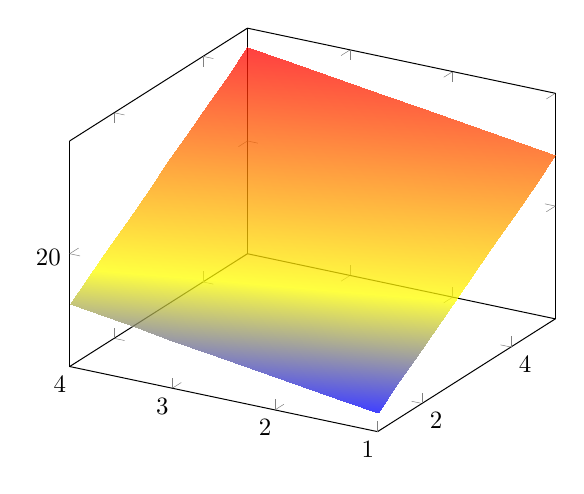
\begin{tikzpicture}[scale=0.9]
        \begin{axis}[view={-60}{30}]
            \addplot3[
                surf,
                domain=1:5,
                domain y=1:4,
                samples=10,
                fill opacity=0.75,
                shader=interp
            ]
            {5*x+2*y};
        \end{axis}
    \end{tikzpicture}
\end{multicols}

\setlength{\columnsep}{-2.0cm}
\begin{multicols}{2}
    \begin{tblr}{vline{1-5}={0mm,solid},
        row{odd}={bg=azure9},
        row{1}={bg=azure3,fg=white,font=\sffamily}}
        \hline[1.25pt]
        nodes & elems & area & bords     \\
        \hline
        1 1   & 0 1 2 & 0    & 0 0 3 1 0 \\
        1 4   & 0 2 3 & 0    & 0 0 1 2 0 \\
        5 4   &       &      & 0 3 2 2 1 \\
        5 1   &       &      & 0 1 2 3 0 \\
        \hline[1.25pt]
    \end{tblr}

    \columnbreak
    \setlength{\leftskip}{1cm}
    \begin{tblr}{vline{1-5} = {0mm,solid},
        row{odd}={bg=azure9},
        row{1}={bg=azure3,fg=white,font=\sffamily}}
        \hline[1.25pt]
        $x$ & $x^*$ & $x^*-x$ & $\|x^*-x\|$    \\
         7.000 &  7.000 &  0.00E+00 &          \\
        13.000 & 13.000 & -9.61E-08 & 3.04E-07 \\
        33.000 & 32.999 &  2.88E-07 &          \\
        27.000 & 27.000 &  0.00E+00 &          \\
        \hline[1.25pt]
    \end{tblr}
\end{multicols}

\subsubsection*{Количество елементов - 4}
\subsubsection*{Количество елементов - 8}
\subsubsection*{Количество елементов - 16}




\subsection*{Тест №3}










\raggedright % Прижать к левому краю
\section{Выводы}
    Выводы

\end{document}



% \renewcommand{\arraystretch}{2}     % Растянуть таблицу
% \renewcommand{\tabcolsep}{5mm}      % Отступы между столбацами
% \centering %  Центрирование


% ~~~~~~~~ INFO ~~~~~~~~ %
% Добавления кода в одну строку
% \inputminted[
% baselinestretch=1.0,
% mathescape=true,
% breaklines,
% linenos
% ]{cpp}{../src/main.cpp}

% Примитивное добавление кода
% \begin{minted}[linenos,mathescape=true,baselinestretch=1.0]{c++}
% #include "argparse/argparse.hpp"
% #include "timer/cxxtimer.hpp"
% #include "LOS/LOS.hpp"
% #include "FEM.hpp"

% int main(int argc, char* argv[]) {
%     using namespace ::Log;
%     using ::std::chrono::milliseconds;

%     argparse::ArgumentParser program("FEM", "1.0.0");
%     program.add_argument("-i", "--input" ).required().help("path to input files" );
%     program.add_argument("-o", "--output").required().help("path to output files");

%     try {
%         program.parse_args(argc, argv);

%         cxxtimer::Timer timer(true);
%         FEM fem      (program.get<std::string>("-i"));
%         fem.writeFile(program.get<std::string>("-o"), 1E-14, 10000);
%         LOS<double> l(program.get<std::string>("-o"));
%         l.solve(Cond::HOLLESKY, true);
%         timer.stop();

%         l.printX();

%         std::cout << '\n' << "Milliseconds: "
%                 << timer.count<milliseconds>() << '\n';
%         fem.printAll();
%         fem.printSparse();
%     }
%     catch(const std::runtime_error& err) {
%         Logger::append(getLog("argc != 3 (FEM -i input -o output)"));
%         std::cerr << err.what();
%         std::cerr << program;
%         std::exit(1);
%     }
%     return 0;
% }
% \end{minted}